%!TEX root = ../thesis.tex
%*******************************************************************************
%****************************** Third Chapter **********************************
%*******************************************************************************
\chapter{Analysis of deep neural networks for predicting DNA methylation} \label{sec:dcpg_ana}

\ifpdf
    \graphicspath{{Chapter5/Figs/Raster/}{Chapter5/Figs/PDF/}{Chapter5/Figs/}}
\else
    \graphicspath{{Chapter5/Figs/Vector/}{Chapter5/Figs/}}
\fi

Deep neural networks are often criticised as hard to interpret `black-box' models. However, model interpretability is critical in multiple fields, including biology and health care. Hence, several approaches have been developed to interpret the parameters of neural networks (\Cref{sec:dl_inter}; \Cref{sec:dl_genomics}) and to obtain insights into learned features. We adapted some of these approaches to analyse DeepCpG (\Cref{sec:dcpg_model}). In particular, we show that DeepCpG can be applied to discover DNA sequence motifs that are associated with methylation states, to identify variance-associated motifs, and to estimate the effect of single nucleotide mutations on DNA methylation. The presented work is based on \citet{angermueller_accurate_2017}.


\section{Discovering DNA sequence motifs} \label{sec:dcpg_ana_motifs}

As described in \cref{sec:dcpg_model}, DeepCpG consists of a DNA, CpG, and joint module. The DNA module has a convolutional architecture with a series of convolutional and max-pooling layers. The filters of the first convolutional layer recognize DNA sequence motifs similarly to conventional position weight matrices and can be visualised as sequence logos (\Cref{sec:dl_genomics}). Existing approaches for visualizing convolutional filters are either \emph{alignment-based} or \emph{optimization-based}. Alignment-based approaches~\citep{alipanahi_predicting_2015,kelley_basset:_2016,quang_danq:_2016} align DNA sequence fragments that maximally activate a certain convolutional filter and visualize the resulting alignment as sequence logo. Optimization-based approaches~\citep{lanchantin_deep_2016,lanchantin_deep_2016-1} optimize the input DNA sequence by gradient descent to maximize the activation of a certain convolutional filter. Our approach is alignment-based. Specifically, we computed the activations $a_{nfi}$ of all filters $f$ of the first convolutional layer for input sequences $s_n$ at every position $i$. We selected sequence window $s_{n,i-L},\ldots,s_{n,i+L}$, if the activation $a_{nfi}$ of filter $f$ with length $L$ at position $i$ (\Cref{eq:dcpg_filter_act}) was greater than 0.5 of the maximum activation of $f$ over all sequences, i.e. $a_{nfi}>0.5 \max_{ni}(a_{nfi})$. We then aligned all selected sequence fragments and visualized filter alignments as sequence logos using WebLogo~\citep{crooks_weblogo:_2004}.

\begin{figure}[htbp!]
\centering
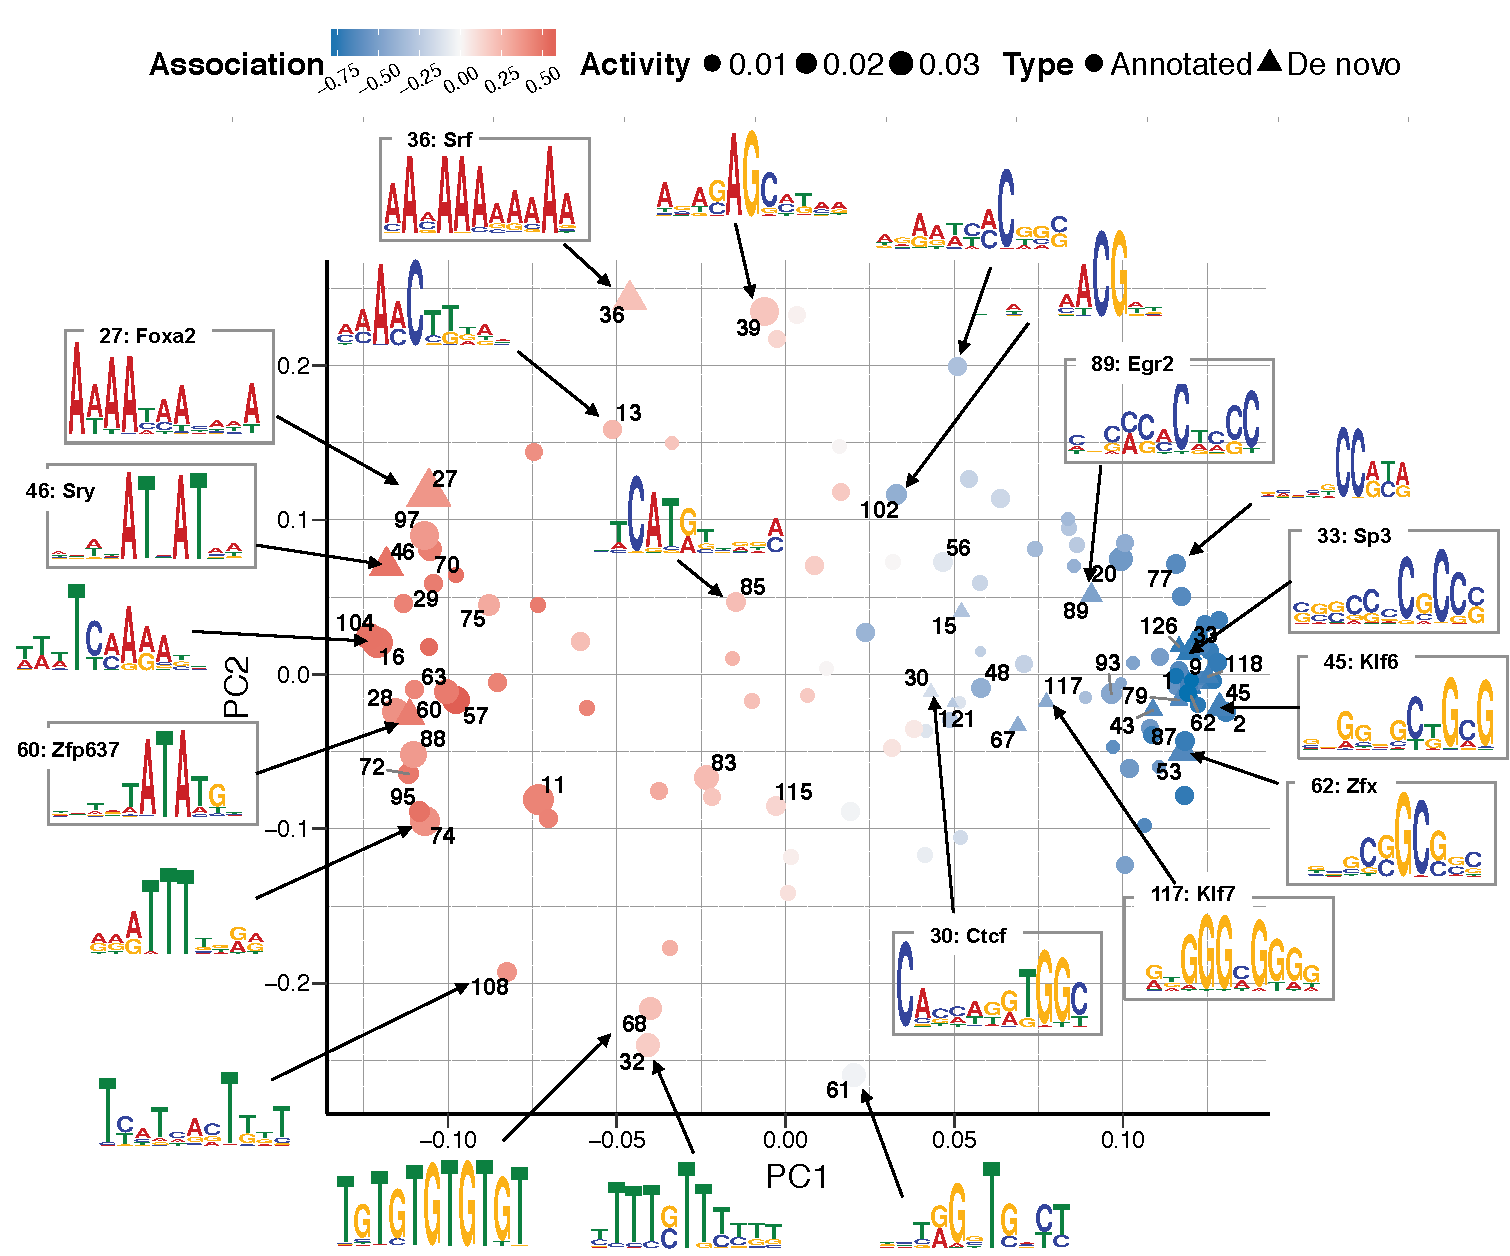
\includegraphics[width=0.9\textwidth]{motifs_pca}
\caption[Principal component analysis of discovered DNA sequence motifs.]{Principal component analysis of discovered DNA sequence motifs. Clustering of 128 motifs discovered by DeepCpG. Shown are the first two principal components of the motif occurrence frequencies in sequence windows (activity). Triangles denote motifs with significant ($\FDR<0.05$) similarity to annotated motif in the CIS-BP or UniPROPE database. Marker size indicates the average activity; the estimated motif effect on methylation level is shown in colour. Sequence logos are shown for representative motifs with larger effects, including 10 annotated motifs.}
\label{fig:dcpg_motifs_pca}
\end{figure}

The number of motifs that the model learns corresponds to the number of convolutional filters, which is a pre-defined hyperparameter. Depending on the choice of this hyperparameter and the nature of the underlying data, learned motifs can be redundant or only weakly associated with DNA methylation. We therefore quantified the importance of learned motifs by two metrics: their activity (occurrence frequency) and their influence on model predictions (association). Specifically, for a set of sequences, e.g. within a certain genomic context, we computed the average of mean sequence activities $\bar{a}_{nf}$, where $\bar{a}_{nf}$ denotes the weighted mean of activities $a_{nfi}$ across all positions $i$ in the sequence window of length $W$:
\begin{align}
  \bar{a}_{nf}=\frac{1}{\sum_{i=1}^W w_i} \sum_{i=1}^W w_i a_{nfi} \qquad w_i=1-\frac{|i-0.5W|}{0.5W}
\end{align}
$w_i$ are linear weights that are highest close the centre position ($i=0.5W$) of the sequence window. We computed the influence of filter $f$ on the predicted methylation states $\hat{y}_{nt}$ of cell $t$ (\Cref{eq:dcpg_y}) as the Pearson correlation $r_{ft}=\operatorname{cor}_n(\bar{a}_{nf},\hat{y}_{nt})$ over CpG sites $n$, and the mean influence $r_f$ over all cells by averaging $r_{ft}$.

\begin{figure}[htbp!]
\centering
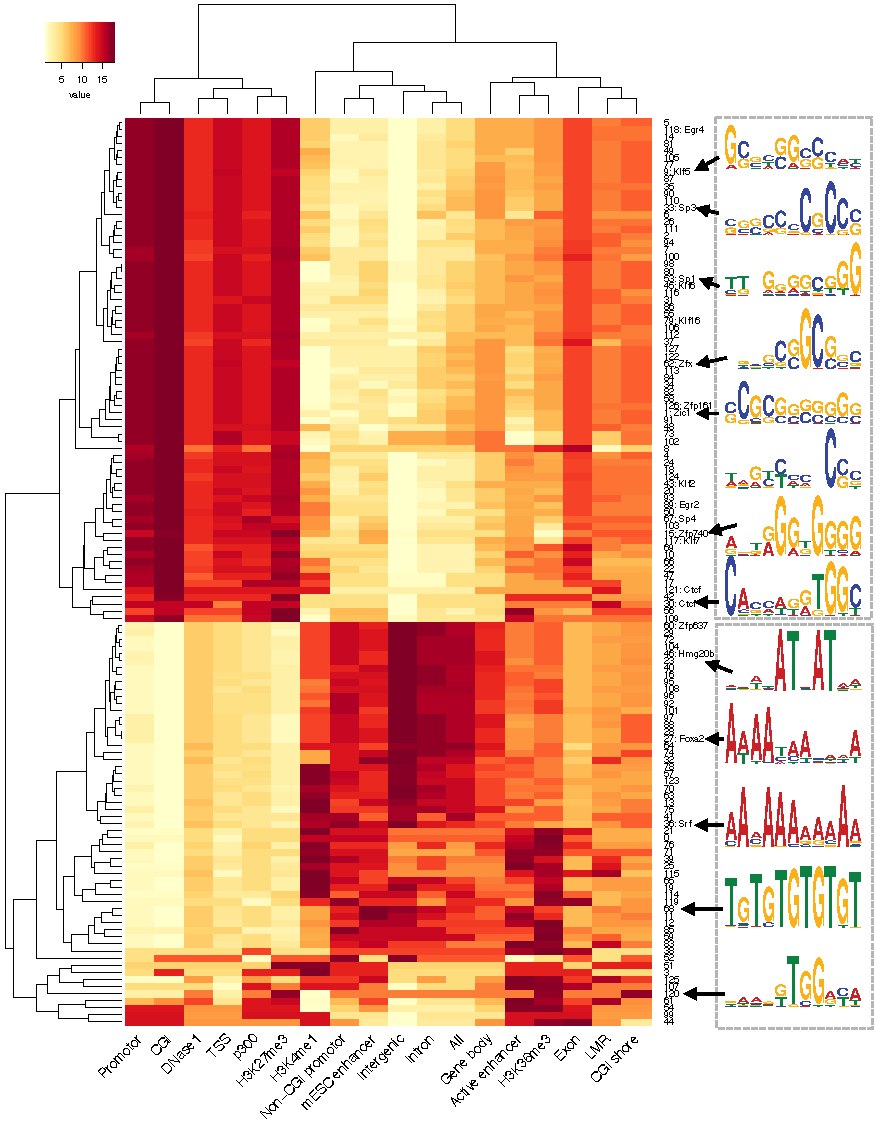
\includegraphics[width=0.8\textwidth]{motifs_act}
\caption[Principal component analysis of discovered DNA sequence motifs.]{Principal component analysis of discovered DNA sequence motifs. Clustering of 128 motifs discovered by DeepCpG. Shown are the first two principal components of the motif occurrence frequencies in sequence windows (activity). Triangles denote motifs with significant ($\FDR<0.05$) similarity to annotated motif in the CIS-BP or UniPROPE database. Marker size indicates the average activity; the estimated motif effect on methylation level is shown in colour. Sequence logos are shown for representative motifs with larger effects, including 10 annotated motifs.}
\label{fig:dcpg_motifs_act}
\end{figure}

To investigate the co-occurrence of motifs across sequence windows, we applied principal component analysis (\Cref{fig:dcpg_motifs_pca}) and hierarchical clustering (\Cref{fig:dcpg_motifs_act}) to motif activities.  Motifs with similar nucleotide composition tended to co-occur in the same sequence windows, where two major motif clusters were associated with increased or decreased methylation levels (\Cref{fig:dcpg_motifs_pca}; \Cref{fig:dcpg_motifs_cor}). Consistent with previous findings~\citep{mendenhall_gc-rich_2010,thomson_cpg_2010,whitaker_predicting_2015}, we observed that motifs associated with decreased methylation tended to be CG rich and were most active in CG rich promoter regions, transcription start sites, as well as in contexts with active promoter marks, such as H3K4me3 or p300 sites (\Cref{fig:dcpg_motifs_act}). Conversely, motifs associated with increased methylation levels tended to be AT rich and were most active in CG poor genomic contexts (\Cref{fig:dcpg_motifs_act}).

We further compared learned motifs, i.e. the weights of the first convolutional layer, to known motifs using Tomtom~\citep{bailey_meme_2009}. 20 out of the 128 learned motifs matched significantly ($\FDR<0.05$) motifs annotated in the Mus Musculus CIS-BP~\citep{weirauch_determination_2014} and UniPROBE~\citep{newburger_uniprobe:_2009} database. 17 of these motifs were transcription factors with a known implication in DNA methylation~\citep{hervouet_dnmt3/transcription_2009,luu_disclosing_2013,whitaker_predicting_2015}, including CTCF~\citep{kim_analysis_2007}, E2f~\citep{tsai_mouse_2008}, and members of the Sp/KLF family~\citep{fernandez-zapico_functional_2011}--transcription factors and regulators of cell differentiation. 13 out of the 20 annotated motifs had been shown to interact with DNMT3a and DNMT3b~\citep{hervouet_dnmt3/transcription_2009}, two major DNA methylation enzymes. Three motifs have no clear associations with DNA methylation. These included Foxa2~\citep{lee_foxa2_2005,wan_compensatory_2005} and Srf~\citep{arsenian_serum_1998,marais_srf_1993}, which are implicated in cell differentiation and embryonic development, as well as Zfp637~\citep{huang_il-6_2016,quenneville_embryonic_2011}, a zinc finger protein that has recently been linked to spermatogenesis in mouse.


\section{Identifying variance-associated motifs}

DNA sequence motifs can either have similar effects in all cells and thereby influence the mean methylation rate across cells, or they can have cell-specific effects and hence account for the variance between cells. Of particular interests for understanding intercellular differences are variance-associated motifs, which we discerned from motifs that are primarily associated with mean methylation levels.

\begin{figure}[htbp!]
\centering
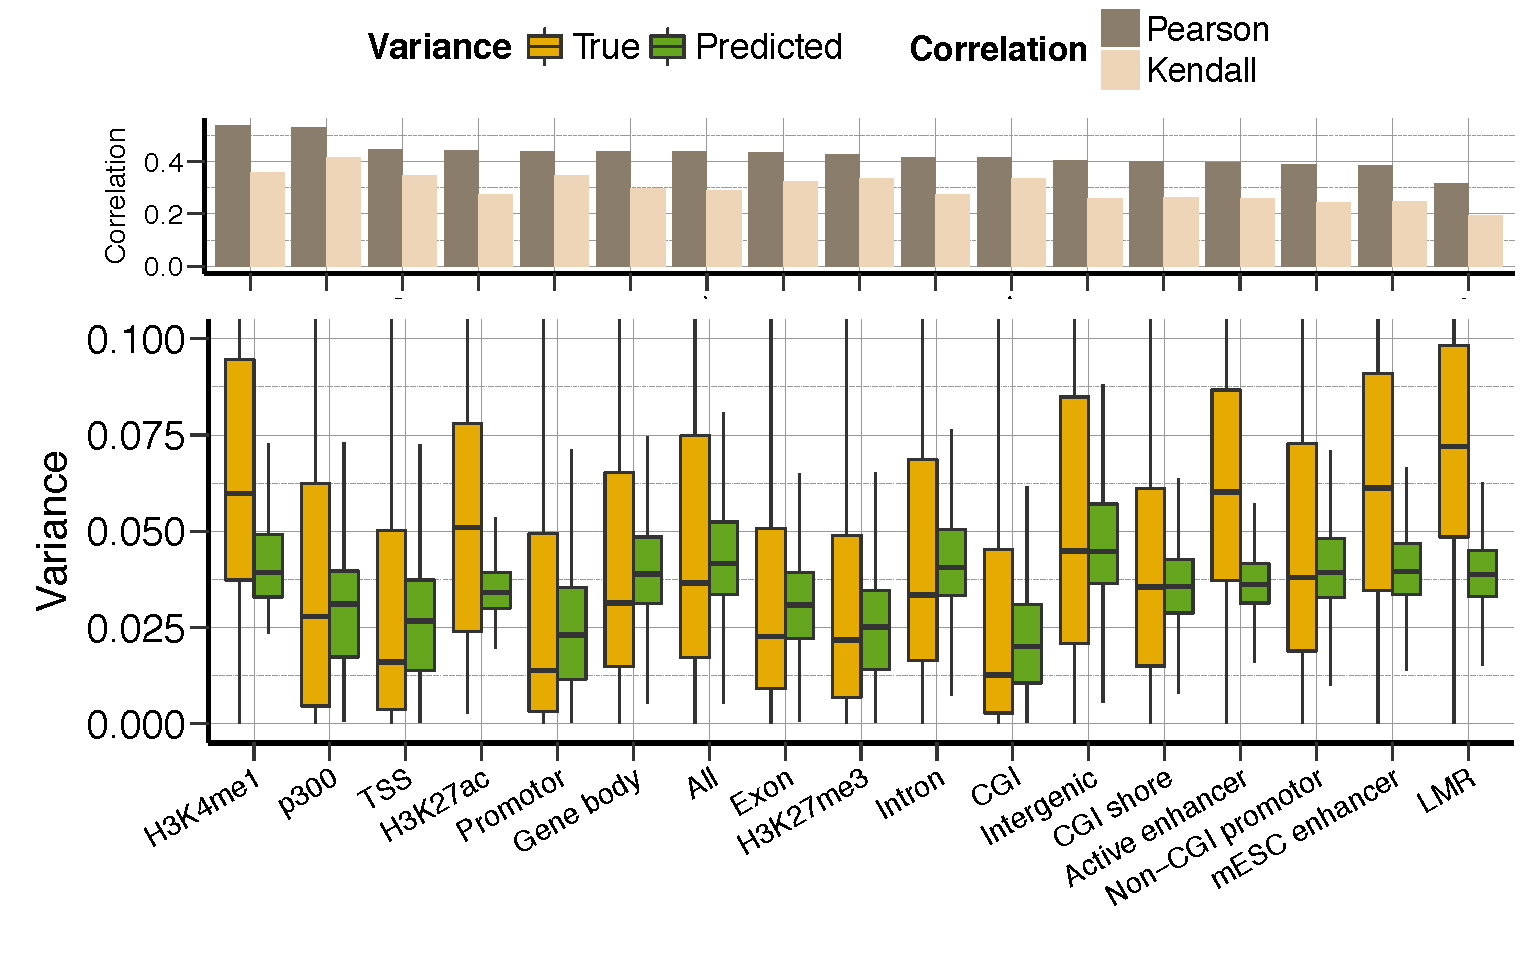
\includegraphics[width=1.0\textwidth]{var_var}
\caption[Performance of DeepCpG DNA module to predict methylation variability.]{Performance of DeepCpG DNA module to predict methylation variability. Boxplot represent predicted (green) and the observed (orange) methylation variability in 3~kbp windows centred on individual CpG sites for different genomic contexts on held out test chromosomes. Barplot represent Pearson and Kendall correlation coefficients.}
\label{fig:dcpg_var_var}
\end{figure}

For this purpose, we trained a second neural network that had the same architecture and in particular reused the motifs from the DNA module of DeepCpG. However, this network was now trained to predict for single CpG sites the variability across cells and the mean methylation rate. Specifically, we replaced output neurons by neurons with a sigmoid activation function to predict for CpG site $n$ both the mean methylation rate $\hat{m}_{ns}$ and cell-to-cell variance $\hat{v}_{ns}$ within a window of size $s\in\{1000,2000,3000,4000,5000\}$~bp. We used multiple window sizes to obtain predictions at different scales, thereby mitigating the uncertainty of mean- and variance estimates in low-coverage regions. For training the resulting model, we initialized and fine-tuned parameters with the corresponding parameters of the DNA module, except for motif parameters of the first convolutional layer. The training objective was
\newcommand{\Xmse}{\operatorname{MSE}}
\begin{align}
  L(w)=\Xmse_w (\hat{m},m,\hat{v},v)+\lambda_2 \norm{w}_2,
\end{align}
where $\Xmse$ the is mean squared error between model predictions and training labels:
\begin{align}
  \Xmse_w(\hat{m},m,\hat{v},v)=\sum_{n=1}^{N}\sum_{s=1}^S (m_{ns}-\hat{m}_{ns})^2+(v_{ns}-\hat{v}_{ns})^2
\end{align}
$m_{ns}$ is the estimated mean methylation rate for a window centred on target site n of a certain size indexed by $s$:
\begin{align}
  m_{ns}=\frac{1}{T}\sum_{t=1}^T m_{nst}
\end{align}
Here, $m_{nst}$ denotes the estimated mean methylation rate of cell $t$ computed by averaging the binary methylation state $y_{it}$ in the set of all observed CpG sites $Y_{nst}$ in window $s$
\begin{align}
  m_{nst}=\frac{1}{|Y_{nst}|} \sum_{i \in Y_{nst}} y_{it},
\end{align}
where $v_{ns}$ denotes the estimated cell-to-cell variance:
\begin{align}
  v_{ns}=\frac{1}{T} \sum_{t=1}^T (m_{nst}-m_{ns})^2
\end{align}
We evaluated this model by holdout validation as we did before (\Cref{sec:dcpg_eval}). Notably, the model could predict both global changes in mean methylation levels (Pearson's $R=0.80$; $\operatorname{MAD}=0.01$; \Cref{fig:dcpg_var_mean}), as well as cell-to-cell variability (Pearson's $R=0.44$; $\operatorname{MAD}=0.03$, \cref{fig:dcpg_var_var}; Kendall's $R=0.29$, \cref{fig:dcpg_var_rank}).

\begin{figure}[htbp!]
\centering
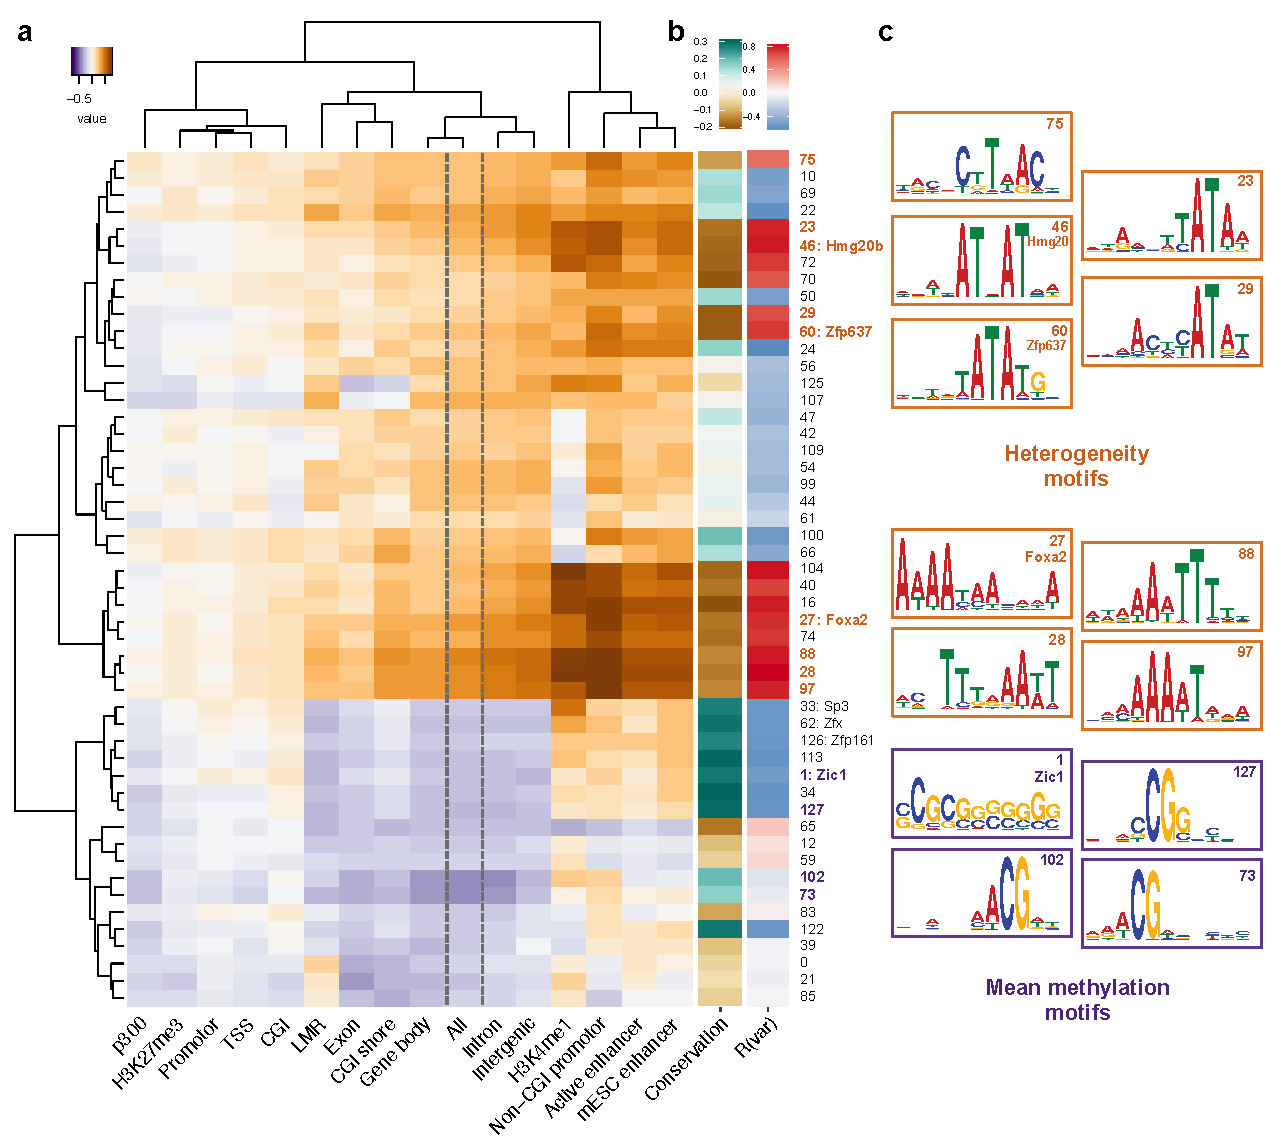
\includegraphics[width=1.0\textwidth]{var_motifs}
\caption[Identification of motifs associated with mean methylation levels and cell-to-cell variability.]{Identification of motifs associated with mean methylation levels and cell-to-cell variability. (a) Difference of motif effect on cell-to-cell variability and methylation levels for different genomic contexts. Motifs associated with increased cell-to-cell variability are highlighted in brown; motifs that were primarily associated with changes in methylation level are shown in purple. (b) Genome-wide correlation coefficients between motif activity and DNA sequence conservation (left), as well as cell-to-cell variability (right). (c) Sequence logos for selected motifs identified in (a), which are highlighted by colour in (b).}
\label{fig:dcpg_var_motifs}
\end{figure}

There is an intrinsic mean-variance relationship of single-cell methylation states (\Cref{fig:dcpg_var_couple}), and hence the separation of the motif impact on mean methylation and methylation variance is partially confounded. To mitigate this effect, we used a scoring approach that separates the effect of individual motifs on cell-to-cell variability and mean methylation levels. Specifically, we computed the influence $r^v_{fs}$ of filter $f$ on cell-to-cell variability in widows of size $s$ as the Pearson correlation between mean sequence filter activities $\bar{a}_{nf}$ and predicted variance levels $\hat{v}_{ns}$ of sites $n$:
\begin{align}
  r^v_{fs}=\operatorname{cor}_n(\bar{a}_{nf},\hat{v}_{ns})
\end{align}
Analogously, we computed the influence $r^m_{fs}$ on predicted mean methylation levels $\hat{m}_{ns}$. We then used the difference $r^d_{fs}=|r^v_{fs}|-|r^m_{fs}|$ between the absolute value of the influence on variance and mean methylation levels to identify motifs that were primarily associated with cell-to-cell variance $r^d_{fs}>0.25$, or with changes in mean methylation levels $r^d_{fs}<-0.25$.

\begin{figure}[htbp!]
\centering
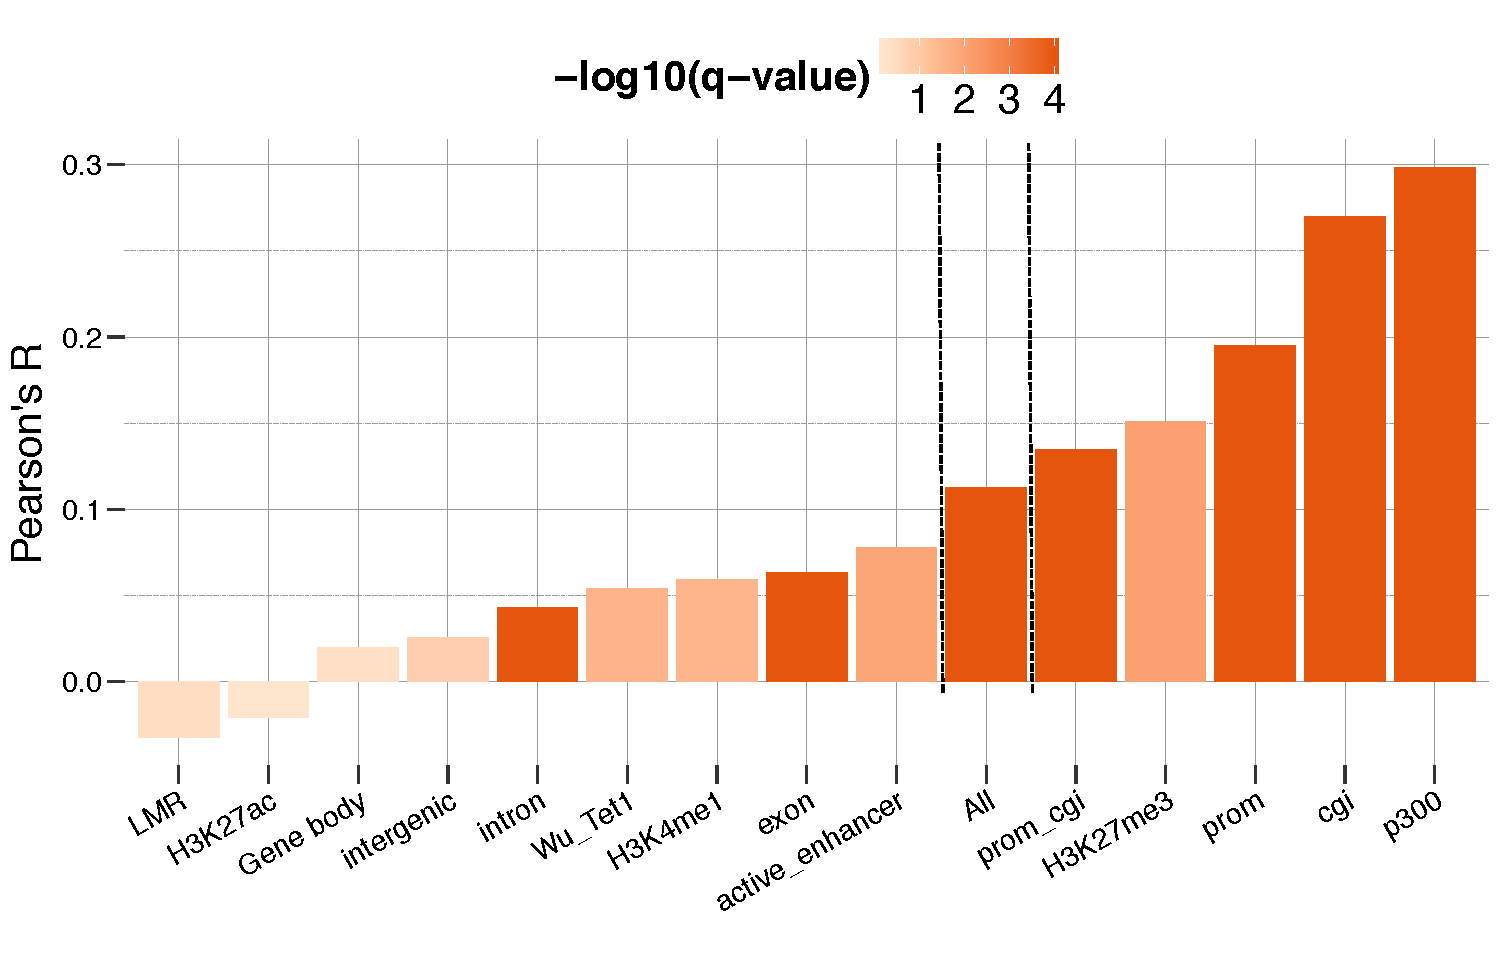
\includegraphics[width=0.8\textwidth]{var_mt}
\caption[Functional assessment of predicted cell-to-cell variability.]{Functional assessment of predicted cell-to-cell variability. Pearson correlation coefficient between methylome-transcriptome linkage as reported in \cref{sec:mt}, and the predicted cell-to-cell variability for test chromosomes. Colour denotes statistical significance (q-value, Benjamini Hochberg adjusted). Significant correlations ($\FDR<0.01$) were observed  genome-wide (`All') and in most genomic contexts.}
\label{fig:dcpg_var_mt}
\end{figure}

The approach identified 22 motifs that were primarily associated with cell-to-cell variance (\Cref{fig:dcpg_var_motifs}). These motifs tended to be active in CG-poor and active enhancer regions--sequence contexts with increased epigenetic variability (\Cref{sec:bs_results}). 12 of the identified motifs were AT-rich and associated with increased variability, including the differentiation factors Foxa2~\citep{lee_foxa2_2005,wan_compensatory_2005}, Hmg20b~\citep{sumoy_hmg20a_2000}, and Zfp637~\citep{huang_il-6_2016,quenneville_embryonic_2011}. Notably, variance-increasing motifs were more frequent in un-conserved regions such as active enhancers, in contrast to variance-decreasing motifs, which were enriched in evolutionary conserved regions such as gene promoters (\Cref{fig:dcpg_var_motifs}~(b); \Cref{fig:dcpg_var_cons}). Our analysis also revealed 4 motifs that were primarily associated with mean methylation levels, which were in contrast CG rich and most active in conserved regions.

To explore whether the model predictions for variable sites are functionally relevant, we overlaid predictions with methylome-transcriptome linkages from our previous study (\Cref{sec:mt}). The rationale behind this approach is that regions with increased methylation variability are more likely to harbour associations with gene expression. Consistent with this hypothesis, we observed a weak but globally significant association (Pearson's $R=0.11$; $P=5.72\times10^-16$; \Cref{fig:dcpg_var_mt}).

\section{Estimating the effect of DNA mutations}

\begin{figure}[htbp!]
\centering
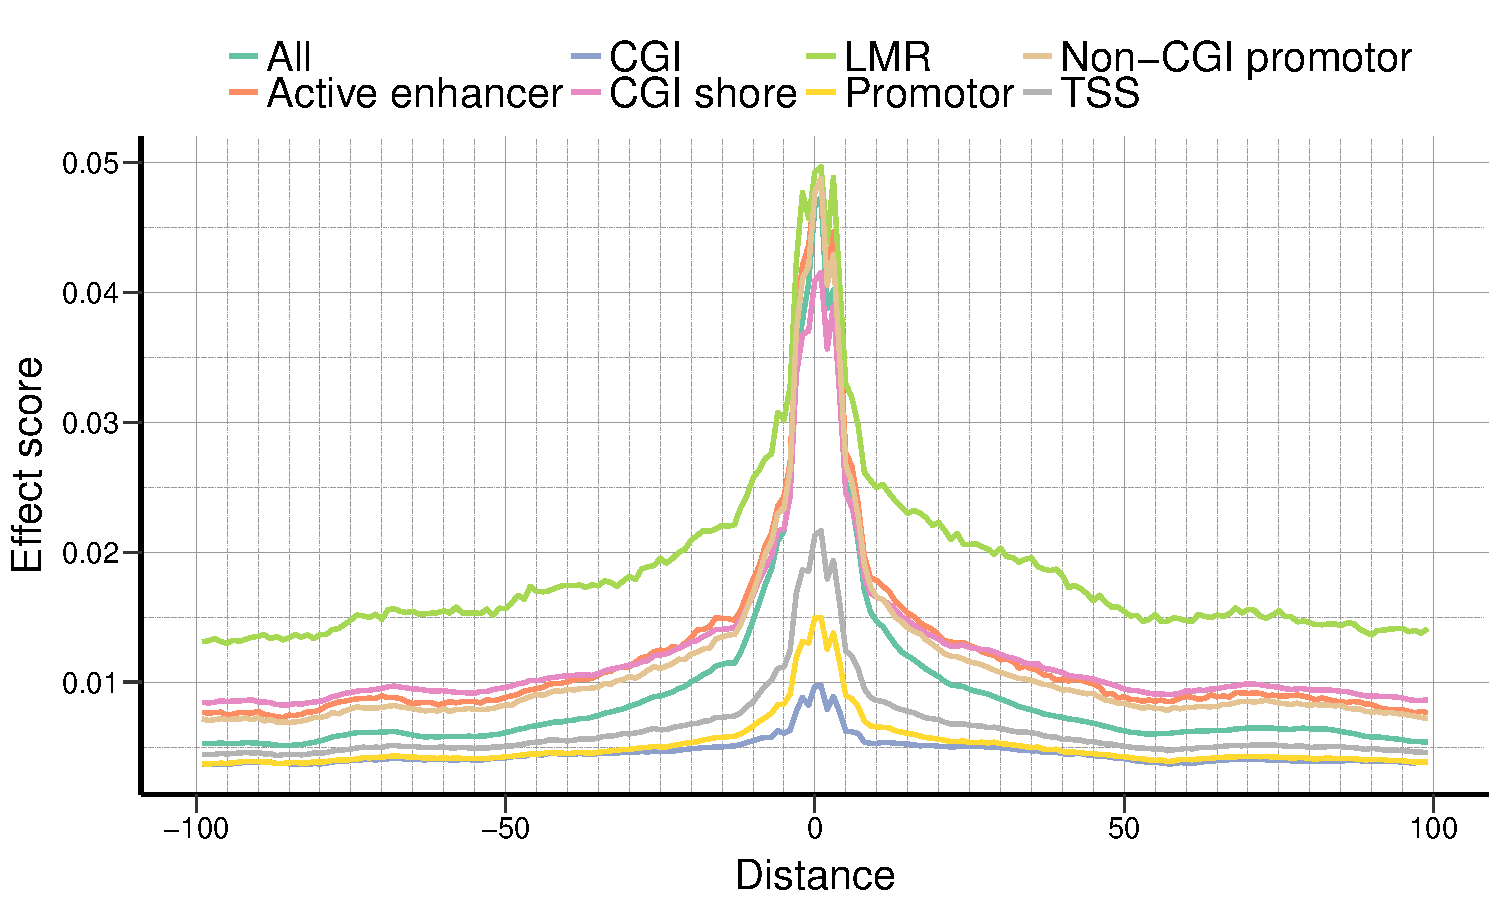
\includegraphics[width=0.9\textwidth]{mut_global}
\caption[Average genome-wide effect of single nucleotide mutations on CpG methylation estimated using DeepCpG.]{Average genome-wide effect of single nucleotide mutations on CpG methylation estimated using DeepCpG, depending on the distance to the CpG site and the genomic context.}
\label{fig:dcpg_mut_global}
\end{figure}

The trained DeepCpG model can also be used to estimate the effect of single nucleotide mutations on CpG methylation. For this purpose, we adapted a gradient-based approach~\citep{simonyan_deep_2013} to estimate mutational effects in a computationally efficient manner, thereby greatly reducing the compute cost compared to previous methods~\citep{alipanahi_predicting_2015,zhou_predicting_2015,zhou_predicting_2015}. Specifically, let $\hat{y}_n(s_n)=\frac{1}{T}\sum_t \hat{y}_{nt}(s_n)$ be the mean predicted methylation rate across cells $t$ for an input sequence $s_n$. Then we quantified the effect $e^s_{nid}$ of changing nucleotide $d$ at position $i$ as:
\begin{align}
  e^s_{nid}=\frac{\Delta \hat{y}_{nt}(s_n)}{\Delta s_{nid}}(1-s_{nid})
\end{align}
Here, the first term is the first-order gradient of $\hat{y}_n$ with respect to $s_{nid}$, and the second term sets the effect of wild-type nucleotides ($s_{nid}=1$) to zero. We quantified the overall effect score $e^s_{ni}$ at position $i$ as the maximum absolute effect over all nucleotide changes, i.e. $e^s_{ni}=\max_d(|e^s_{nid}|)$.

\begin{figure}[htbp!]
\centering
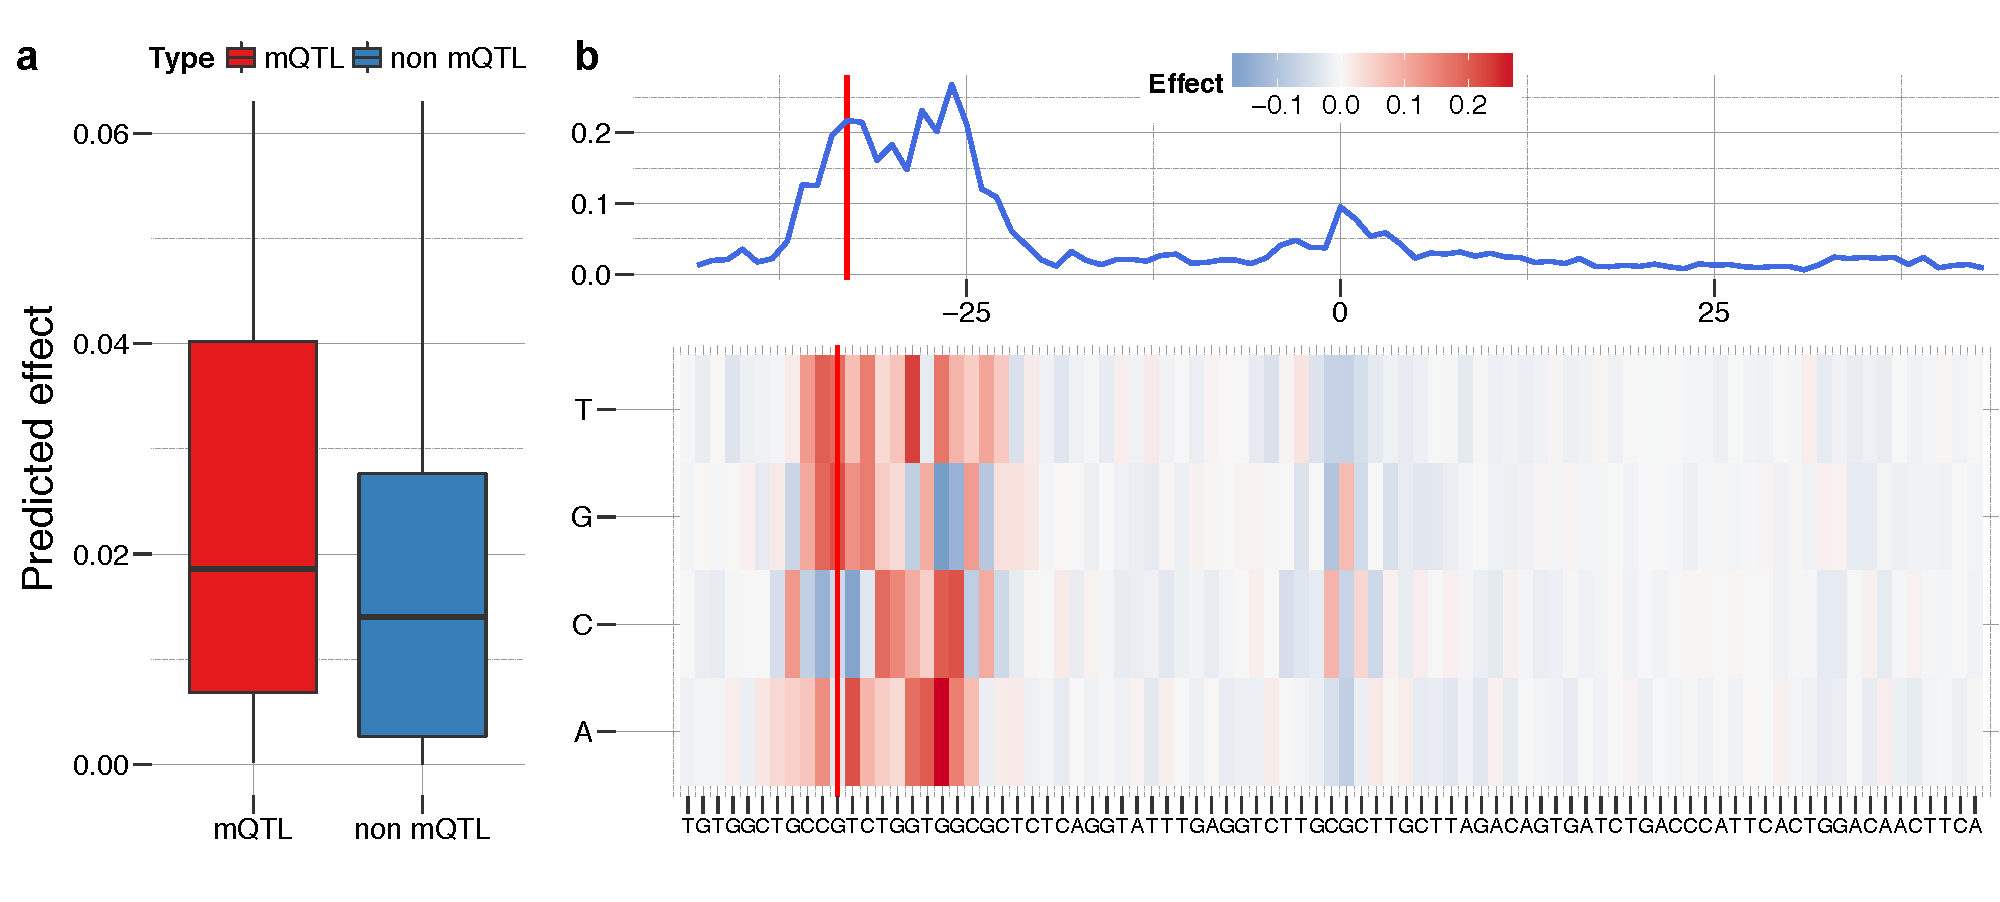
\includegraphics[width=1.0\textwidth]{mut_qtl_zoom}
\caption[Analysis and example visualization of estimated single nucleotide mutation effects for methylation QTLs.]{Analysis and example visualization of estimated single nucleotide mutation effects for methylation QTLs. (a) Distribution of the mutation effect for 2379 methylation QTLs (mQTL) variants from \citet{kaplow_pooling-based_2015}, compared to distance-matched random variants (non mQTL). (b) Visualization of mutation effects for an example CpG site and the corresponding mQTL. Shown are effects in a window centred on the example CpG site (chromosome 1; position 159791497). The position of the corresponding mQTL from \citet{kaplow_pooling-based_2015} (rs60205880; position 159791464) is indicated by the vertical red line. The heat map in the lower panels shows effect sizes for individual nucleotides, and line plot in the upper panel the maximum absolute effect across nucleotides.}
\label{fig:dcpg_mut_qtl_zoom}
\end{figure}

As expected, mutations in the direct vicinity of the target CpG site had the largest effects (\Cref{fig:dcpg_mut_global}). Mutations in CG dense regions such as CGIs or promoters tended to have smaller effects, suggesting that DNA methylation in these genomic contexts is more robust to single nucleotide mutations. Globally, we observed a negative correlation between mutational effects and DNA sequence conservation ($P<1.0\times10^{-15}$; \Cref{fig:dcpg_mut_cons}), providing evidence that estimated single nucleotide effects capture genuine effects.

We further evaluated mutational effects by comparing the effect for 2379 methylation QTLs (mQTLs) from \citet{kaplow_pooling-based_2015} with the effect for matched non-mQTL variants. Since \citet{kaplow_pooling-based_2015} mapped mQTLs in human cells, we used the DeepCpG model trained on HepG2 cells for this experiments. To adjust of differences in effect due to the distance to the CpG site (\Cref{fig:dcpg_mut_global}), we randomly sampled non-QTLs at distances matched to mQTLs. Known mQTL variants had significantly larger effects than matched random variants ($P<1.0\times10^{-15}$, Wilcoxon rank sum test; \Cref{fig:dcpg_mut_qtl_zoom}), providing evidence that DeepCpG can be used to identify functional variants from the DNA sequence alone.


\section{Discussion}

We have developed alternative approaches for interpreting the parameters of DeepCpG and for obtaining insights into the learned features. We have used these approaches to discover motifs that are associated with DNA methylation states, to identify variance-associated motifs, and to estimate the effect of single nucleotide mutations on DNA methylation.

Although our approaches helped to better understand DeepCpG, they are not free of limitations. First, the randomness that is involved in the training of DeepCpG affects which specific motifs are learned. This applies in particular to the random initialization of the parameters of the first convolutional layer. One way to address this problem is to initialize a fraction of convolutional filters by known DNA sequence motifs, which, however, can introduce biases and decrease prediction accuracy.

Although our approaches helped to better understand DeepCpG, they are not free of limitations. First, the randomness that is involved in the training of DeepCpG affects which specific motifs are learned. This applies in particular to the random initialization of the parameters of the first convolutional layer. One way to address this problem is to initialize a fraction of convolutional filters by known DNA sequence motifs, which, however, requires prior knowledge about methylation-associated motifs for the cell type of interest and can introduce biases.

Second, the model can learn redundant and overlapping motifs depending on the choice of the number of convolutional filters and the dropout rate. More distinct motifs can be obtained by penalizing the number motifs with non-zero weights, analogously to the Bayesian automatic relevance determination framework~\citep{mackay_bayesian_1992,neal_bayesian_2012}.

Third, our scoring approach to identify variance-associated motifs does not fully disentangle the mean-variance relationship of binomial-distributed methylation states in single cells. One approach to more clearly separate between mean and variance motifs would be to model methylation states using a beta-binomial distribution, where mean and over-dispersion parameters are predicted by a deep neural network, similar to mixture density networks~\citep{bishop1994mixture}.

Forth, our gradient-based approach to quantify the effect of single nucleotide mutations is problematic because the ReLU activation function can have a gradient of zero but still transfer information. This problem has recently been addressed by comparing neuron activations to reference activations~\citep{shrikumar_not_2016}--a promising strategy also in the context of DNA methylation. Another avenue of future research is to quantify statistical significance of estimated effect scores, which is important for prioritizing genomic variants.
